%!TEX root = ../MasterThesis.tex

\section{Collaboration on \gls{E-commerce} fraud incidents}
\label{sec:concept_overview}

Based on the explanations in Chapter~\ref{cha:context_analysis}, and especially the scope definition for this Master Thesis in Section~\ref{sec:scope_thesis}, the collaborative system for investigating \gls{E-commerce} fraud incidents has to answer the central question:\@

\begin{quotation}
  \textit{Is this transaction really a valid \gls{E-commerce} transaction?}
\end{quotation}

Looking into the stakeholders, who can provide useful information to decide it, one will come up with:\@

\begin{enumerate}
    \item \textbf{Merchants}, who can provide additional information of each \gls{E-commerce} transaction in question.
    \item \textbf{\gls{PSP}s/issuers}, who have information about the credit card usage patterns and the original credit card owners.
    \item \textbf{\gls{LSP}s}, who can offer information about whether an order has already been shipped or not, and in the former case to whom it has been handed over.
\end{enumerate}

Ideally, each of those participants would make parts of their internal databases available for the others to access and query for information in a shared information space. That would allow those stakeholders, who have to authorize or validate a suspicious credit card transaction, to analyse all available information as depicted in the Figure~\ref{fig:images_system_overview}.\@

\begin{figure}[H]
	\centering
		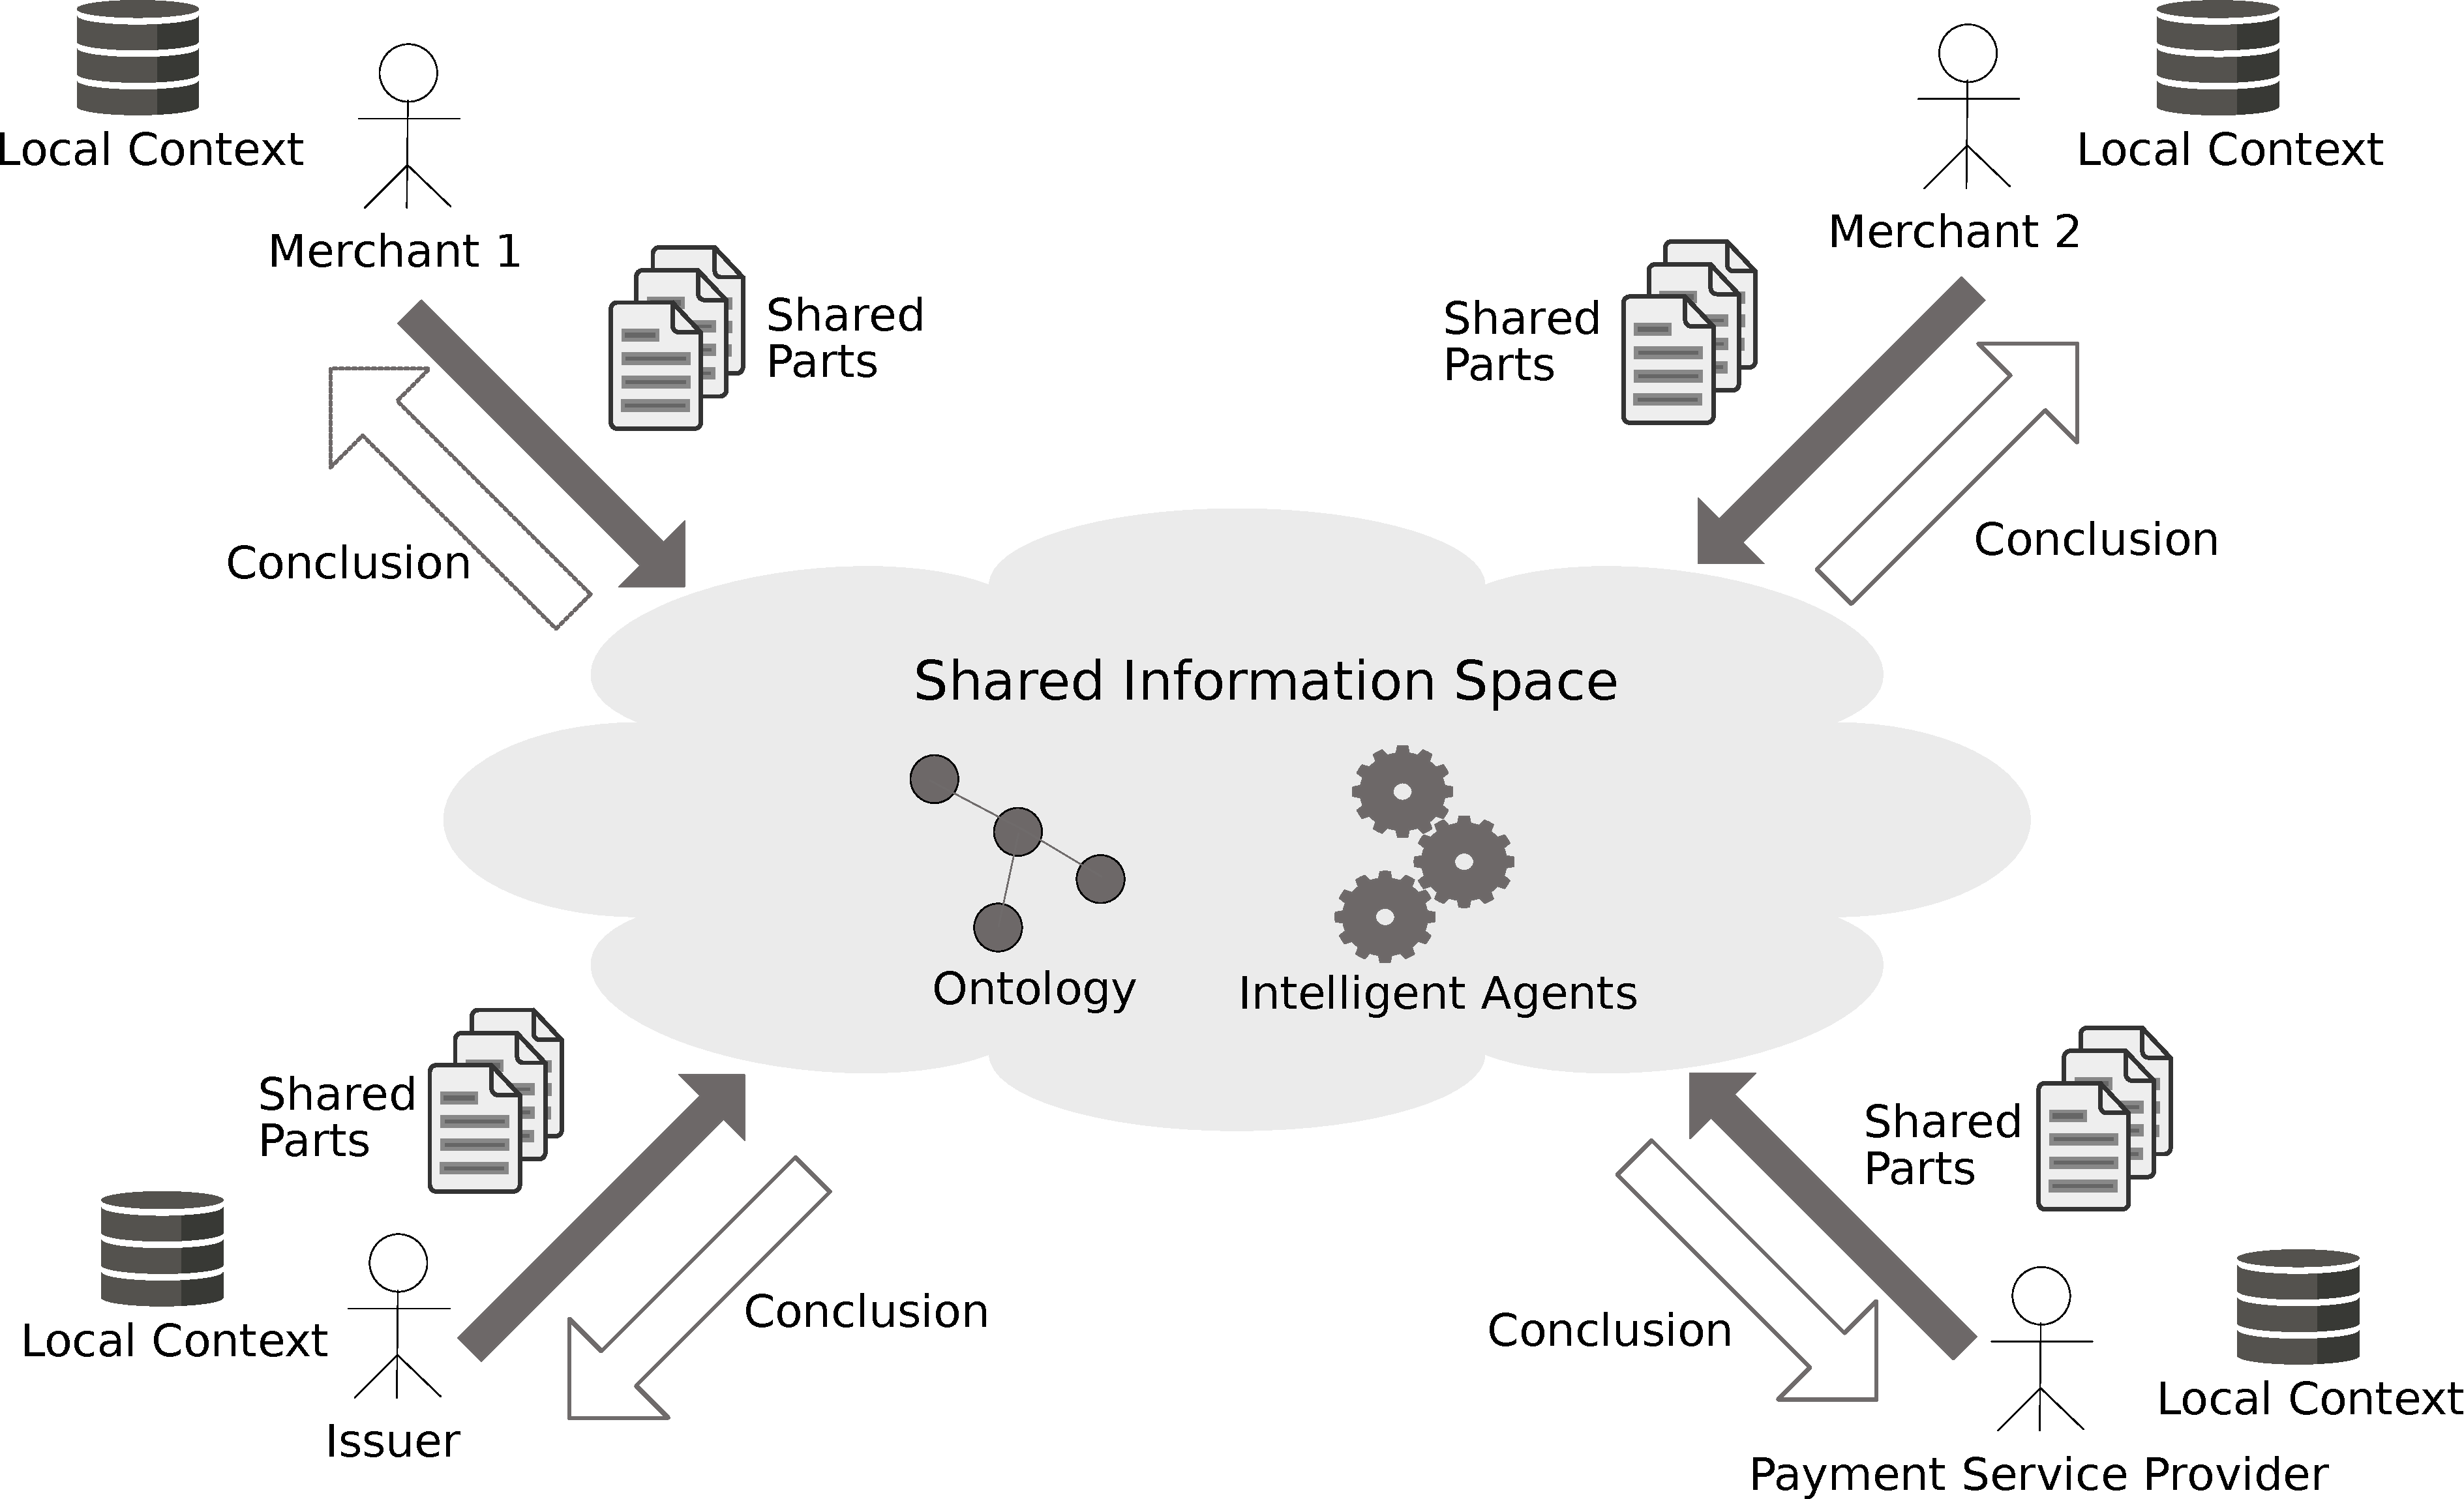
\includegraphics[width=0.9\columnwidth]{images/system_overview.pdf}
	\caption{High-level concept of the system}
\label{fig:images_system_overview}
\end{figure}

In this figure one can see, how the relevant parties provide access to parts of their internal local context information within a shared information space. The collaborative system should allow participants to communicate and collaborate on the \gls{E-commerce} fraud incidents from different places at the same time (see Section~\ref{sec:cscw}). Due to the fact that data from various sources have to be combined into a shared understanding of the \gls{E-commerce} activities of a consumer, there is a need to harmonise and transform the information from each participant into a common data model to be able to analyse the combined data set. Based on the shared understanding of the \gls{E-commerce} activities that have been done with a credit card recently, a set of intelligent agents (aka analysis tools) can assess them and present their findings, which can be valuable to any of the participants of the collaborative system.

% section concept_overview end
